\chapter{Research Design and Implementation}
\label{ch:research_design_and_implementation}
This chapter will discuss the motivation, design and implementation of the \acrshort{slr}.
The chapter is structured as follows.
In \cref{sec:research_motivation} the impact and usefulness of the study is argued.
\cref{sec:research_questions} presents the research questions of the study.
\cref{sec:research_method} outlines the research method and design of the study.
Finally, \cref{sec:research_implementation} accounts for how the study was conducted.

\section{Research Motivation}
\label{sec:research_motivation}
As outlined in \cref{ch:background}, industry adoption of \acrshort{ml} is still in its early stages and rapidly growing.
The \acrshort{se} aspect of \acrshort{ml} is an active field of research, with the vast majority of work having been done only in the past five years.
As reported by earlier literature studies in the field (see \cref{ch:related_work}), operationalization of \acrshort{ml} is an area which presents practitioners with real challenges, such as how to deliver model artifacts to the production environment or how to monitor evolving input data \cite{Paleyes2020}.
Tackling operationalization challenges requires adopting good practices as well as utilizing suitable tooling.
Earlier work has largely had a broad scope, with goals of mapping out general \acrshort{se} challenges and practices for \acrshort{ml}.
In short, this study is motivated by two key factors.
\begin{itemize}
    \item Researching \acrshort{ml} operationalization in-depth, and not as part of a broader study of \acrshort{se} for \acrshort{ml}.
    \item Putting more focus on tooling and infrastructure by identifying how current tools are used and what is reported to need further research.
\end{itemize}

\section{Research Questions}
\label{sec:research_questions}
The overarching research question of this study is "\textbf{What is the state of the art in \acrshort{ml} deployment?}".
The focus will be on tooling and trying to identify feature gaps reported in studies where model deployment is discussed.
To support the main research question, four subquestions have been defined:
\begin{itemize}
    \item \textbf{RQ1: How are ML models operationalized in the state of the art?}
    \item \textbf{RQ2: What are the main challenges in operationalizing ML models?}
    \item \textbf{RQ3: What tools and software infrastructure are used to operationalize ML models?}
    \item \textbf{RQ4: What are the feature gaps in the tooling and infrastructure used to operationalize ML models?}
\end{itemize}
The working definition of \emph{operationalization} in this paper is outlined in \cref{sec:deploying_ml_systems}.

\section{Research Method and Design}
\label{sec:research_method}
This study is a \acrfull{slr} based on the guidelines of \textcite{Kitchenham07guidelinesfor} and \textcite{Wohlin2014}.
In this section, the research methodology, i.e. review protocol, will be described.

\subsection{Search Strategy}
Typically, candidate papers in an \acrshort{slr} are identified by constructing a search string for querying digital libraries.
However, initial string-based searches (using strings such as "machine learning deployment", "MLOps deployment", etc) in Oria in late September 2021 failed to produce adequately relevant articles for the topic at hand.
The articles found did not report deployment details related to the operationalization aspect of \acrshort{se} for \acrshort{ml} that this study is concerned with.
This motivated the use of snowballing as an alternative approach for identifying candidate papers.
The snowballing procedure followed the process proposed by \textcite{Wohlin2014}, with the exception that forward and backward snowballing were limited to a single iteration each.
Forward snowballing will be conducted using the \emph{Cited by} functionality of Google Scholar\footnote{\url{https://scholar.google.com/}}.

\subsection{Study Selection}
Studies will be selected based on the criteria found in \cref{tab:selection_criteria}.
Inclusion requires that the study satisfies all of the inclusion criteria, while fulfilling only one of the exclusion criteria leads to exclusion.
The year 2015 was chosen as earliest year of publication as this was when research on \acrshort{se} for \acrshort{ml} began to gain traction \cite{Kumeno2020}, possibly in part due to \textcite{Sculley2015}.
\begin{table}[h]
    \centering
    \begin{tabular}{l|p{0.8\linewidth}}
    Inclusion criteria &  Written in English \\
    & Published in a peer-reviewed journal, conference or workshop \\
    & Published after 2015\\
    & Discusses one of the following aspects of \acrshort{ml} operationalization: challenges, solutions, tooling, processes, requirements \\
    & Available online\\
    \hline
    Exclusion criteria & One of the inclusion criteria is not satisfied\\
    \end{tabular}
    \caption{Study selection criteria used in the \acrshort{slr}.}
    \label{tab:selection_criteria}
\end{table}

\subsection{Study Quality Assessment}
The quality of included studies will be assessed using the criteria found in \cref{tab:study_quality_criteria}, adapted from criteria used by \cite{Giray2021} and suggested by \cite{Garousi2016}.
Studies are subject to assessment criteria marked with \emph{X} depending on whether or not they are empirical.
For each criterion, the study is awarded 1 point for \emph{yes}, 0.5 for \emph{partly} and 0 for \emph{no}.
Sources with an average of 0.5 points or less are excluded.

\begin{table}[]
    \centering
    \begin{tabular}{l c c}
        Criteria & Empirical & Non-empirical \\
        \hline
        Does the author have authority on the subject? & X & X \\
        Does the source have a clearly stated aim? & X & X \\
        Is the author free of any vested interests? & X & X \\
        Have key related sources been linked to or discussed? & X & X \\
        Is relevance (to industry or academia) discussed? & X & X \\
        Does the source have a stated methodology? & X &  \\
        Are any threats to validity clearly stated? & X & \\
    \end{tabular}
    \caption{Study quality assessment criteria for empirical and non-empirical sources, indicated by \emph{X}. Based on criteria from \cite{Garousi2016} and \cite{Giray2021}.}
    \label{tab:study_quality_criteria}
\end{table}

\subsection{Data Extraction}
\label{sec:method:data_extraction}
In order to answer the research questions, sufficient data must be gathered from the literature.
Thus, the data extraction form found in \cref{tab:data_extraction_form} was designed.
Each field is marked by the research question(s) they are intended to facilitate in answering.

\begin{table}[]
    \centering
    \begin{tabular}{l|p{8.5cm}}
        Field & Explanation\\
        \hline
        Author & Name of author(s)  \\
        Publication year & Year of publication \\
        Context & Description of context where necessary \\
        Achievement & Main achievement of the study \\
        Process & Description of the operationalization process (RQ1) \\
        Tools \& infrastructure & Tools and infrastructure used for operationalization (RQ1, RQ3) \\
        Challenges & Operationalization challenges reported (RQ2) \\
        Solutions & Implemented or proposed solutions to reported problems (RQ1, RQ2) \\
        Requirements & Reported requirements for operationalization process, tooling and infrastructure (RQ4) \\
        Gaps & Reported unmet requirements, open problems and proposed research directions in infrastructure or tooling  (RQ4) \\
        Other & Any other notes \\
    \end{tabular}
    \caption{Data extraction form with clarification of the content for each field.}
    \label{tab:data_extraction_form}
\end{table}

\subsection{Data Synthesis}
\label{sec:data_synthesis_method}
Data synthesis will be done through the use of thematic analysis as described in \cite{Lochmiller2021}.
A simplified version of the procedure will be used based on the relatively small dataset and the researcher's inexperience with qualitative methods.
A single cycle of coding will be performed (rather than multiple), followed by reviewing possible themes and finally attempting to articulate the findings.

\section{Research Implementation}
\label{sec:research_implementation}
Selection, quality assessment and data extraction was conducted in an online spreadsheet\footnote{\url{https://docs.google.com/spreadsheets/d/1VMBLQZBsc5dgldnDfHH8cHAWk9ikjxX0TVq4lfYbMpg/edit?usp=sharing}}.

\subsection{Search}
In order to start the snowballing, an initial set of studies was assembled.
The studies were mainly found through the reference lists of earlier related work, such as \cite{John2021} and \cite{MartinezFernandez2021}.
Some manual search with Google Scholar was also done using search strings such as "Mlops deployment" and "machine learning deployment".
The start set can be found in \cref{tab:complete_start_set}.

The study selection criteria found in \cref{tab:selection_criteria} were applied to the start set.
From the start set of 19 papers, 8 satisfied the selection criteria and minimum study quality score, and were thus selected for review and further snowballing.
The papers selected from the start set can be found in \cref{tab:selected_start_set}.

Backward snowballing from the 8 selected papers provided an additional 21 candidate papers based on skimming title/abstract/content of all referred papers from the start set.
Of the 21 candidate papers, 6 papers satisfied the selection criteria and minimum study quality criteria.
The papers selected from backward snowballing can be found in \cref{tab:selected_backward_snowballing}.

Forward snowballing from the start set yielded 29 initial candidate papers.
After applying selection criteria, 10 candidate papers remained, of which all satisfied the minimum study quality criteria.
The papers selected from forward snowballing can be found in \cref{tab:selected_forward_snowballing}.

The total number of papers to review was thus 24.

\begin{table}[]
    \centering
    \begin{tabular}{l|p{0.6\textwidth}}
        Study & Title \\
        \hline
        \textcite{Hazelwood2018} & \citetitle{Hazelwood2018} \\
        \textcite{Hummer2019} & \citetitle{Hummer2019} \\
        \textcite{Krishnamurthi2019} & \citetitle{Krishnamurthi2019}\\
        \textcite{Liu2020} & \citetitle{Liu2020}\\
        \textcite{Chen2020} & \citetitle{Chen2020}\\
        \textcite{Bosch2021} & \citetitle{Bosch2021}\\
        \textcite{Ruf2021} & \citetitle{Ruf2021}\\
        \textcite{Granlund2021} & \citetitle{Granlund2021}\\
    \end{tabular}
    \caption{Studies selected from start set.}
    \label{tab:selected_start_set}
\end{table}

\begin{table}[]
    \centering
    \begin{tabular}{l|p{0.6\textwidth}}
        Study & Title \\
        \hline
        \textcite{Li2017} & \citetitle{Li2017} \\
        \textcite{Baylor2017} & \citetitle{Baylor2017} \\
        \textcite{Crankshaw2017} & \citetitle{Crankshaw2017} \\
        \textcite{Lwakatare2019} & \citetitle{Lwakatare2019} \\
        \textcite{Bernardi2019} & \citetitle{Bernardi2019} \\
        \textcite{Garcia2020} & \citetitle{Garcia2020} \\
    \end{tabular}
    \caption{Studies selected from backward snowballing.}
    \label{tab:selected_backward_snowballing}
\end{table}

\begin{table}[]
    \centering
    \begin{tabular}{l|p{0.6\textwidth}}
        Study & Title \\
        \hline
        \textcite{Yadwadkar2019} & \citetitle{Yadwadkar2019} \\
        \textcite{Rausch2019} & \citetitle{Rausch2019} \\
        \textcite{Rausch2019a} & \citetitle{Rausch2019a} \\
        \textcite{Peticolas2019} & \citetitle{Peticolas2019} \\
        \textcite{Chahal2020} & \citetitle{Chahal2020} \\
        \textcite{Zhang2020} & \citetitle{Zhang2020} \\
        \textcite{Paeaekkoenen2020} & \citetitle{Paeaekkoenen2020} \\
        \textcite{Gupta2020} & \citetitle{Gupta2020} \\
        \textcite{Richins2020} & \citetitle{Richins2020} \\
        \textcite{Choi2021} & \citetitle{Choi2021} \\
    \end{tabular}
    \caption{Studies selected from forward snowballing.}
    \label{tab:selected_forward_snowballing}
\end{table}

\subsection{Data Extraction}
Data extraction proceeded by reading the literature and extracting information as described in \cref{sec:method:data_extraction} and entering the data in a spreadsheet.

\subsection{Data Synthesis}
Data synthesis with thematic analysis was performed as described in \cref{sec:data_synthesis_method} with the help of TreeSheets\footnote{\url{https://strlen.com/treesheets/}}, a hierarchical spreadsheet application.
For each research question, relevant extracted data for each author was entered in the hierarchy.
The data pieces were then coded according to their content.
Lastly, the hierarchy swap feature was used to reorganize the data from being author-oriented to being code-oriented, which enabled discovery of commonalities and differences between studies.
An example of this is shown in \cref{fig:hierarchy_swap}.
\begin{figure}
\centering
\begin{subfigure}[b]{0.45\textwidth}
    \centering
    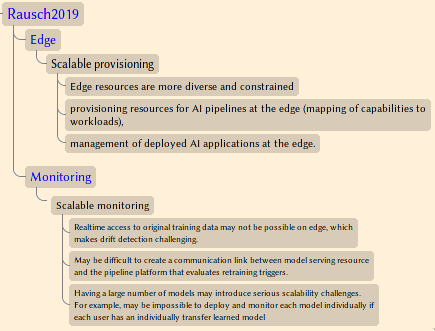
\includegraphics[width=\textwidth]{figures/author-oriented.png}
    \caption{Example of author-oriented data using \cite{Rausch2019} as an example.}
    \label{fig:author-oriented}
\end{subfigure}
\hfill
\begin{subfigure}[b]{0.45\textwidth}
    \centering
    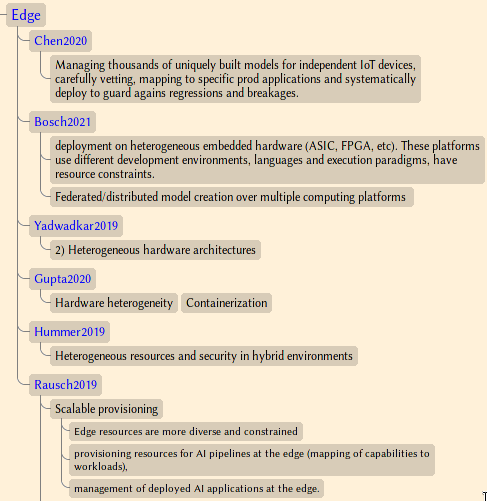
\includegraphics[width=\textwidth]{figures/code-oriented.png}
    \caption{Example of code-oriented data related to edge deployments.}
    \label{fig:code-oriented}
\end{subfigure}
\hfill
\caption{Illustration of hierarchy swap in the coding process. In \cref{fig:author-oriented}, the data is author-oriented after initial coding. After applying the hierarchy-swap feature, data is clustered by the \emph{Edge} code in \cref{fig:code-oriented}.}
\label{fig:hierarchy_swap}
\end{figure}
    